% A skeleton file for producing Computer Engineering reports
% https://kgcoe-git.rit.edu/jgm6496/KGCOEReport_template

\documentclass[CMPE]{../KGCOEReport}

% The following should be changed to represent your personal information
\newcommand{\classCode}{CMPE 460}  % 4 char code with number
\newcommand{\name}{Andrei Tumbar}
\newcommand{\LabSectionNum}{2}
\newcommand{\LabInstructor}{Beato}
\newcommand{\TAs}{Xavier Brooks\\
Diana Yakobchuk\\
Charles Poliwoda}
\newcommand{\LectureSectionNum}{1}
\newcommand{\LectureInstructor}{Beato}
\newcommand{\exerciseNumber}{8}
\newcommand{\exerciseDescription}{Heartbeat Monitor}
\newcommand{\dateDone}{April 1st}
\newcommand{\dateSubmitted}{April 17th}

\usepackage{tikz}
\usepackage{circuitikz}
\usetikzlibrary{calc}
\usetikzlibrary{circuits.logic.IEC,calc}
\usepackage{multirow}
\usepackage{float}
\usepackage[T1]{fontenc}
\usepackage{lmodern}
\usepackage{siunitx}
\usepackage{subcaption}
\usepackage{graphicx}
\usepackage[usestackEOL]{stackengine}
\usepackage{scalerel}
\usepackage{amsmath}
\usepackage{pdfpages}

\sisetup{math-micro=\text{µ},text-micro=µ}

\ctikzset{logic ports=ieee}

\def\lbar#1{\ThisStyle{%
    \setbox0=\hbox{$\SavedStyle#1$}%
    \stackengine{2.2\LMpt}{$\SavedStyle#1$}{\rule{\wd0}{0.1\LMpt}}{O}{c}{F}{F}{S}%
}}

\DeclareFontFamily{U}{mathx}{\hyphenchar\font45}
\DeclareFontShape{U}{mathx}{m}{n}{ <-> mathx10 }{}
\DeclareSymbolFont{mathx}{U}{mathx}{m}{n}
\DeclareFontSubstitution{U}{mathx}{m}{n}
\DeclareMathAccent{\widebar}{\mathalpha}{mathx}{"73}

\makeatletter
\newcommand{\cwidebar}[2][0]{{\mathpalette\@cwidebar{{#1}{#2}}}}
\newcommand{\@cwidebar}[2]{\@cwideb@r{#1}#2}
\newcommand{\@cwideb@r}[3]{%
    \sbox\z@{$\m@th\mkern-#2mu#3\mkern#2mu$}%
    \widebar{\box\z@}%
}
\newcommand\currentcoordinate{\the\tikz@lastxsaved,\the\tikz@lastysaved}
\makeatother

\newcommand\decbin[9]{%
    \par\smallskip
    \makebox[3cm][r]{$#1$\ }\fbox{#2}\,\fbox{#3}\,\fbox{#4}\,\fbox{#5}\,\fbox{#6}\,\fbox{#7}\,\fbox{#8}\,\fbox{#9}\par}


\def\code#1{\texttt{#1}}

\ctikzset{resistors/scale=0.8}

\ctikzset{logic ports/scale=0.7}

\begin{document}
    \maketitle
    \section*{Abstract}

    In this laboratory exercise a simple heartbeat monitor circuit was modeled and
    constructed on a breadboard. The heartbeat monitor operated on a signal from
    an optoisolator circuit or a signal generator mimicking this sensor.
    The purpose of the circuit was to filter a desired
    signal from a noisy input. Choosing the appropriate frequency ranges to filter
    out of an input signal with the goal of sending a measurable analog signal to the
    MSP432 microcontroller. Finally a PCB was designed and laid out as well as an order
    made to a manufacturer.

    \section*{Design Methodology}

	The heart rate monitor circuit is able to measure a low frequency periodic signal
	in the presence of noise. An optoisolator circuit is used to detect a heart beat
	in the neck or wrist. Small variations in the reflection of light against the
	OBP745 can be detected in the generated signal of the optoisolator.

	\begin{figure}[h!]
        \centering
        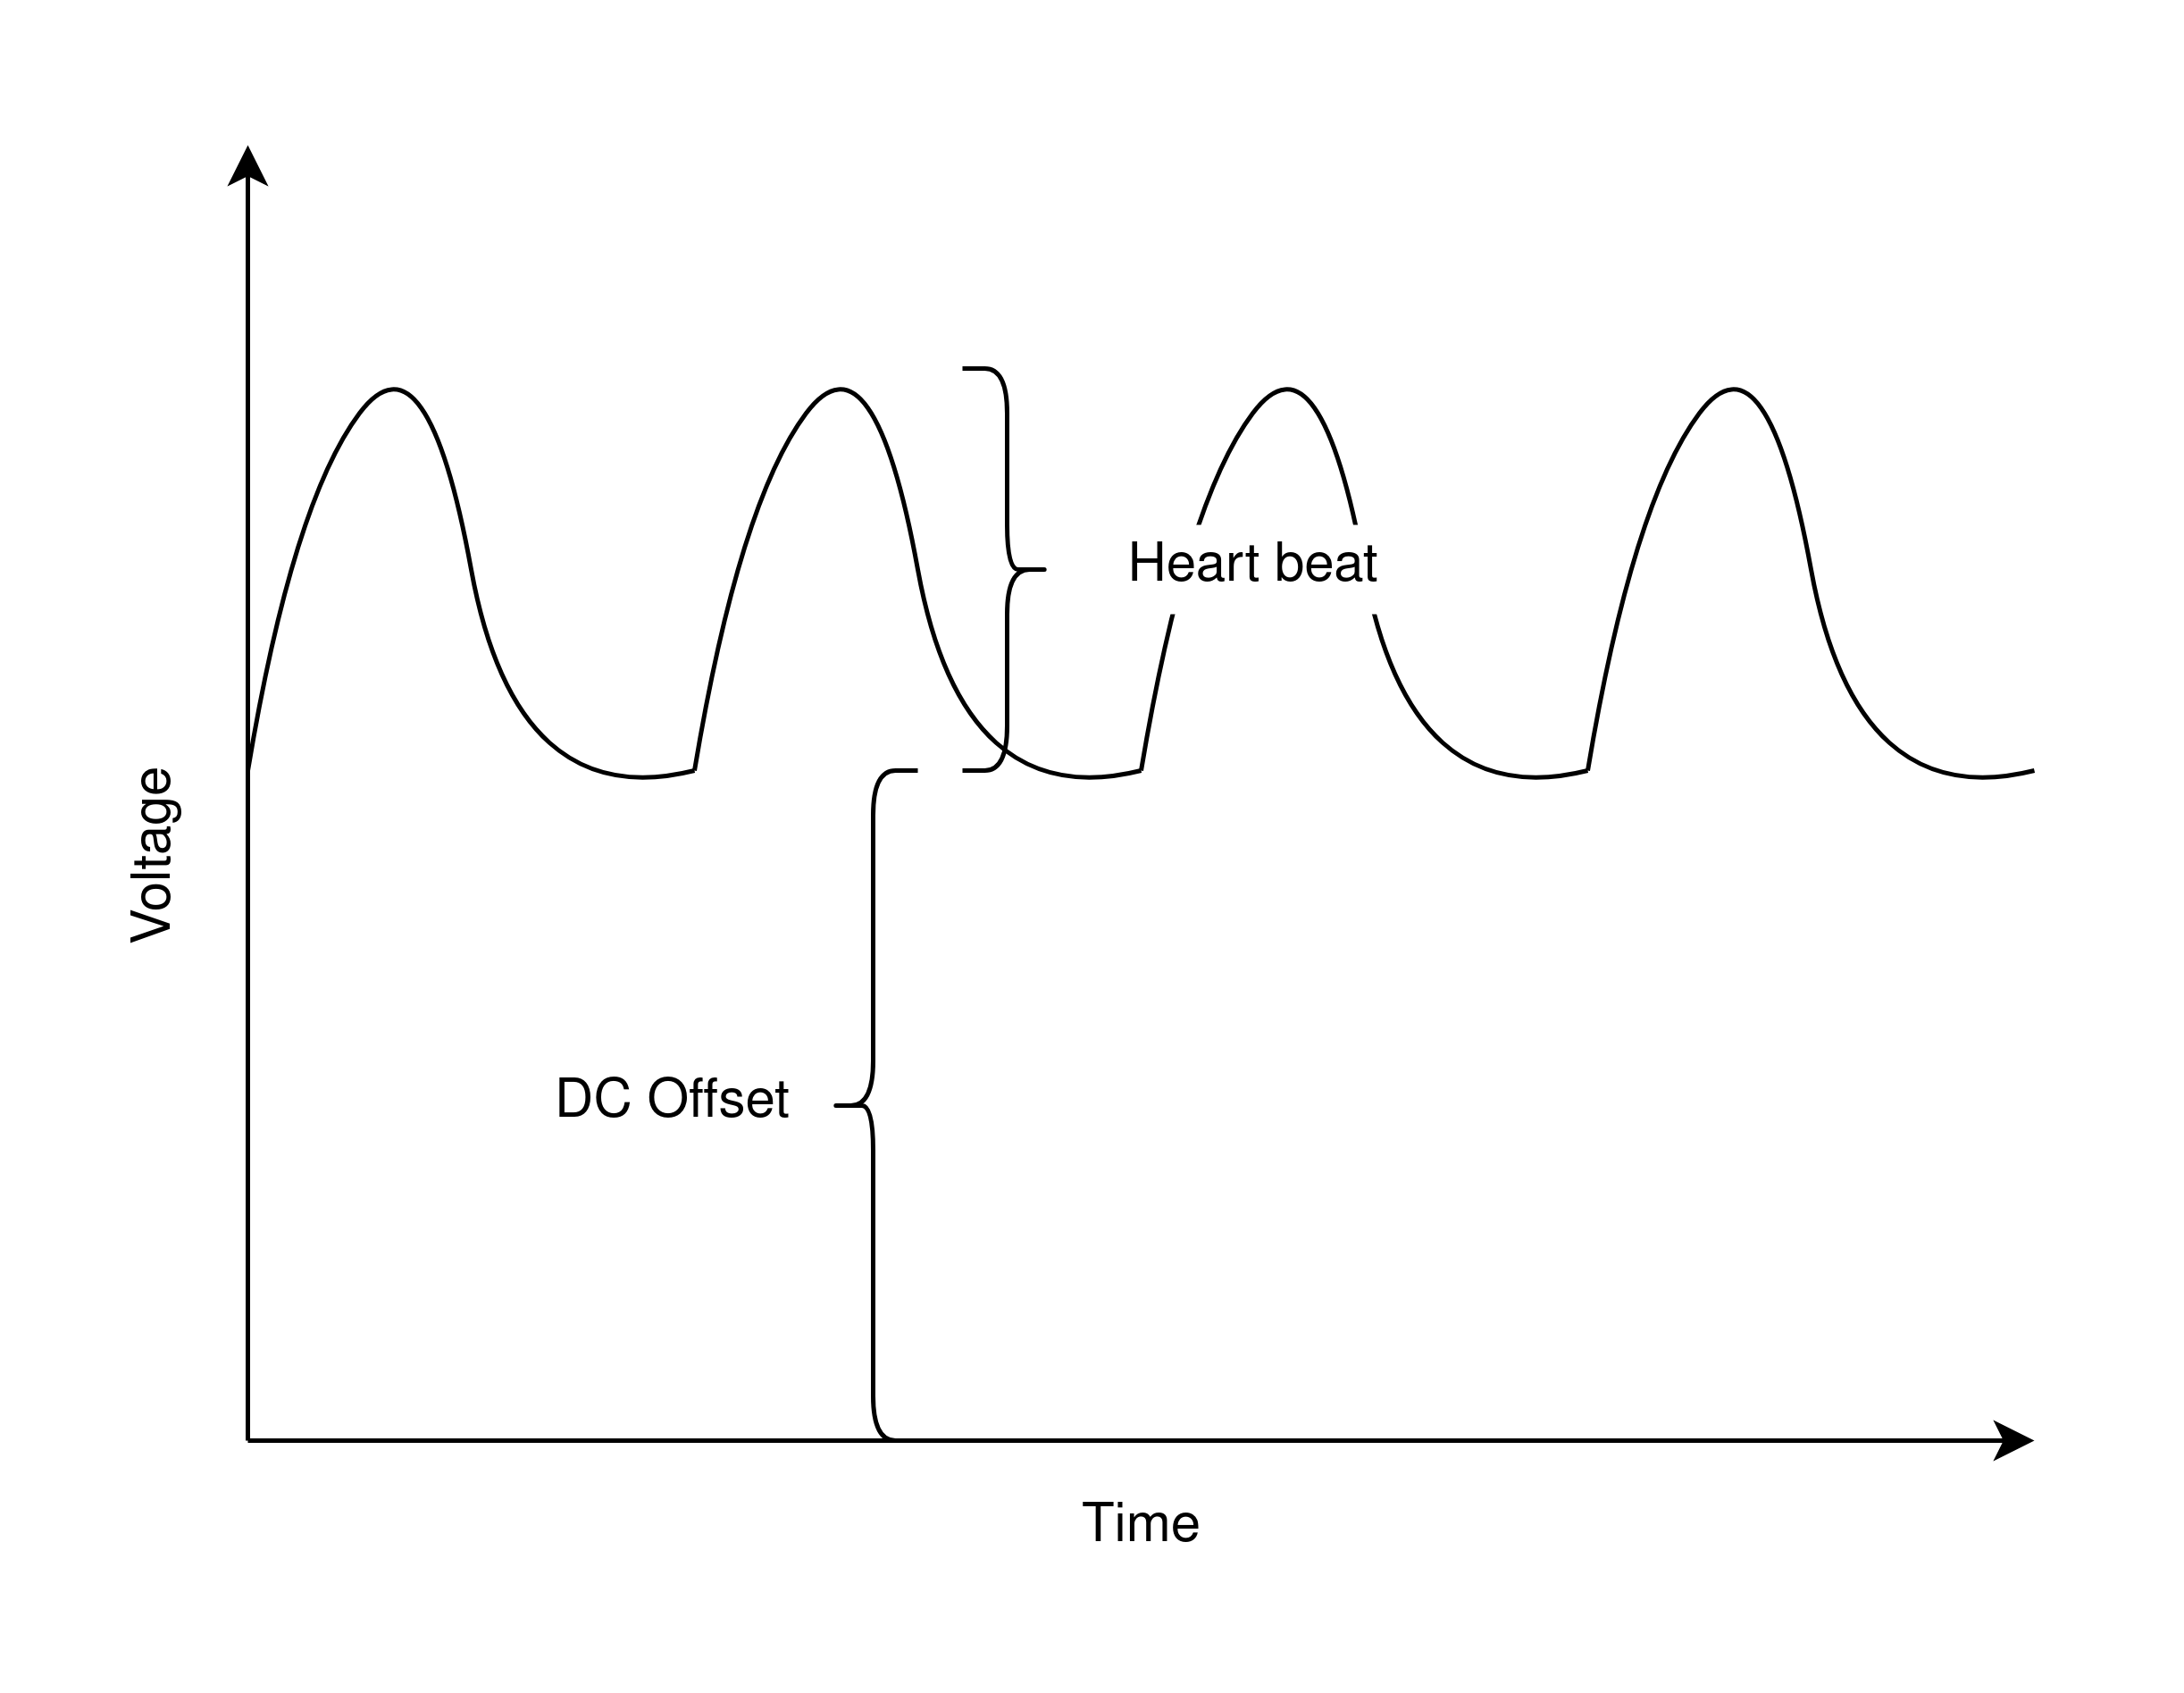
\includegraphics[width=12cm]{heartbeat}
        \caption{Example heartbeat signal from an optoisolator circuit.}
        \label{fig:heartbeat}
	\end{figure}

	Figure \ref{fig:heartbeat} shows an example of the signal generated by an optoisolator
	circuit if it were to be held up to the neck or wrist. Notice that the signal has a
	DC offset which comes from the fact that the heart beat signal will only vary the
	base voltage being output from the optoisolator. Figure \ref{fig:heartbeat} also
	does not show the noise from the optoisolator which would show up as higher frequency
	signals. High amount of noise will make the signal undetectable if it were directly
	fed into the microcontroller. Another challenge from the raw signal of the optoisolator
	is the amplitude of the wave itself. At an amplitude of about \SI{35}{\milli\volt},
	the signal is very difficult to detect on the microcontroller which accepts signals
	from \SI{0}{\volt} to its \SI{2.5}{\volt} reference. \\

	All of these problems may be solved by filtering the signal generated by the
	optoisolator. The DC offset is in fact a \SI{0}{\hertz} signal and may be filtered
	out with a high-pass filter. The signal after a high pass filter with a relatively
	small cut-off frequency will look similar to the signal shown in Figure 
	\ref{fig:heartbeat},
	however it will not include the DC offset. The next issue is static noise. Static noise
	can be characterized as a signal with constant magnitude across all frequencies.
	Because our desired signal is of relatively low frequency when comparing the the
	frequency spectrum of static noise, the higher frequency noise will cause the signal
	to appear "fuzzy". To
	filter out this feature from the signal, a low-pass filter may be used. Choosing the
	correct cut-off frequencies for both the low-pass and the high-pass is key in
	designing the heartbeat monitor circuit.

	\subsection*{Low pass filter}
	While the average beats-per-minute of the heart may vary from person to person
	\cite{b1}, the maximum heart rate of humans is usually based on age. The older a
	person gets, the lower their maximum heartrate. At 20 years of age, the maximum
	heartrate is about 200 bpm \cite{b2}. While this number influences the cutoff
	frequency of the low-pass filter, 200 bpm (\SI{3.33}{\hertz}) should not be directly
	used as the cut off frequency. Firstly, the cut-off frequency is simply the
	\SI{-3}{\dB} point of the transfer function. This means that frequencies above this
	range will not be completely cut off. Another thing to consider is the fact that
	after the two filters, we must apply a voltage gain to scale the signal to a voltage
	range that is detectable by the microcontroller. Ideally, frequencies out of the
	range of the human heartbeat should not be amplified. For this reason, a lower
	frequency of \SI{2}{\hertz} was chosen as a low-pass cut-off frequency.

	\subsection*{High pass filter}
	The cutoff frequency of the high pass filter should be low enough to not cut
	off the desired signal, but also high enough to to properly filter out the DC offset.
	A frequency of \SI{0.5}{\hertz} was chosen for this purpose.

	\subsection*{Schematic \& Simulation}

	As previously discussed, the heartbeat monitor circuit consists of a high-pass filter,
	followed by a low-pass filter, followed by a gain stage. The circuit for the optoisolator
	is discussed in \cite{b4} and will be used as the input into our filter stages.

	\pagebreak

	\begin{figure}[h!]
        \centering
        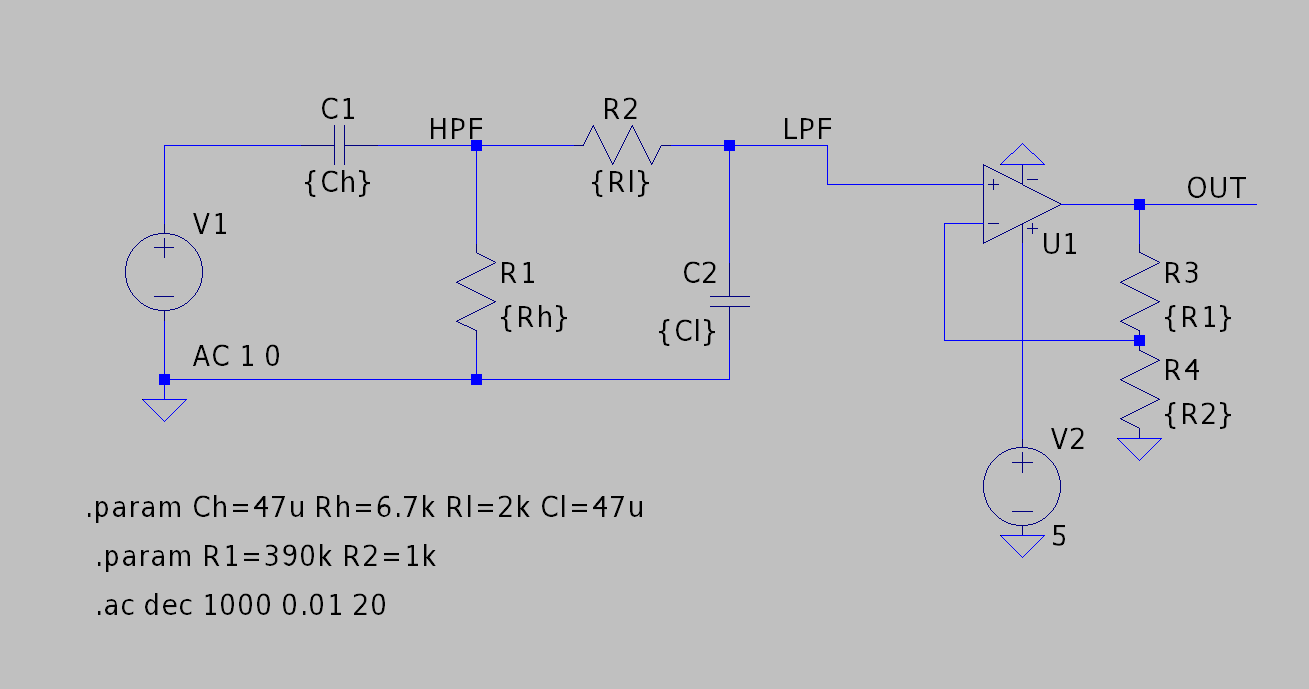
\includegraphics[width=12cm]{schematic}
        \caption{Schematic layout of heartbeat monitor.}
        \label{fig:schematic}
	\end{figure}

	As seen in Figure \ref{fig:schematic}, the values chosen for the resistors and
	capacitors in high and low pass filters will yield cutoff frequencies of
	\SI{.505}{\hertz} and \SI{1.693}{\hertz} respectively.
	These numbers are slightly off from the chosen cutoff frequencies due to resistor
	and capacitor availability in the lab. Finally, the gain stage is meant
	gain the filtered optoisolator signal from \SI{35}{\milli\volt} to about
	\SI{3}{\volt}. This schematic layout was simulated in LTSpice to find the ideal
	gain of the signal across frequencies ranging from \SI{10}{\milli\hertz} to
	\SI{20}{\hertz}.

	 \begin{figure}[h!]
        \centering
        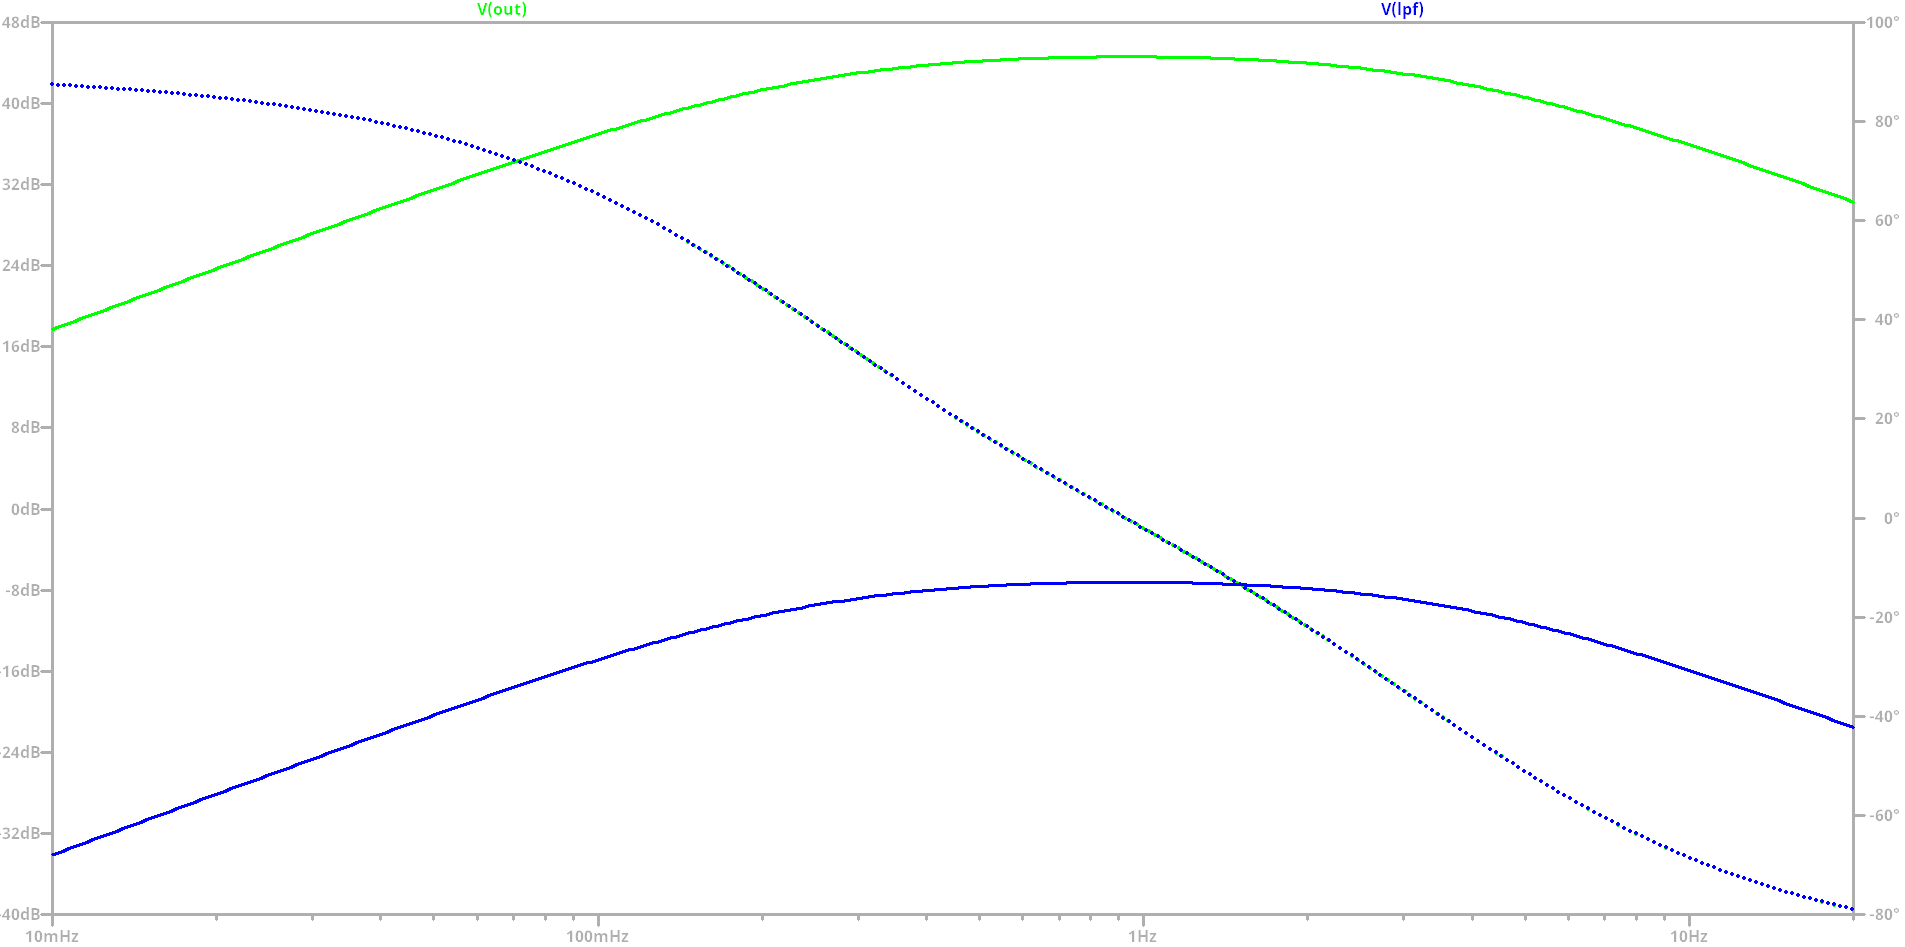
\includegraphics[width=12cm]{transfer}
        \caption{Transfer function of heartbeat monitor circuit from
        \SI{10}{\milli\hertz} to \SI{20}{\hertz} between all filter stages.}
        \label{fig:transfer}
	\end{figure}

	Figure \ref{fig:transfer} shows the transfer function of the heartbeat sensor
	plotted across relevant frequencies. The plot shows the transfer function for the
	output of each individual filter stage as well as for the overall circuit including
	the gain stage. We can see that at about \SI{1}{\hertz}, the circuit is applying
	about \SI{44}{\dB} gain on the signal. If we convert that to linear gain, we find
	that this op-amp configuration will multiple the voltage by about 158 times.

	\begin{align}
	\SI{44}{\dB} &= 20log(A_{linear})\\
	A_{linear} &\approx 158\\
	V_{in} &= \SI{35}{\milli\volt}\\
	V_{out} &\approx \SI{2.5}{\volt}\\
	\frac{V_{out}}{V_{in}} &= 72 \neq 158
	\end{align}

	Looking at the equations above, the expected signal magnitude from the optoisolator
	is about \SI{35}{\milli\volt} and the desired voltage should be amplified to use
	a good portion of the range of the analog to digital converter (ADC).
	The MSP432's ADC has a reference voltage of
	\SI{2.5}{\volt} meaning any voltage above this range will be cut off to the maximum
	digital output of the ADC. The theoretical gain required to amplify a
	\SI{35}{\milli\volt} signal to \SI{2.5}{\volt} is 72 (linear). However, because in
	reality we are not using ideal components, we will see a decrease in amplification
	as tolerance variations will cause a delta compared to simulation.
	A linear gain of 158 is used in this circuit as it showed great results.

    \section*{Results \& Analysis}

	To test the functionality of the circuit, an oscilloscope capture was taken
	on the output node following each of the three stages (high-pass, low-pass, gain).
	A sinusoidal input signal from the signal generator was used with a
	\SI{500}{\milli\volt} DC offset and \SI{35}{\milli\volt} amplitude.

	\begin{figure}[h!]
        \centering
        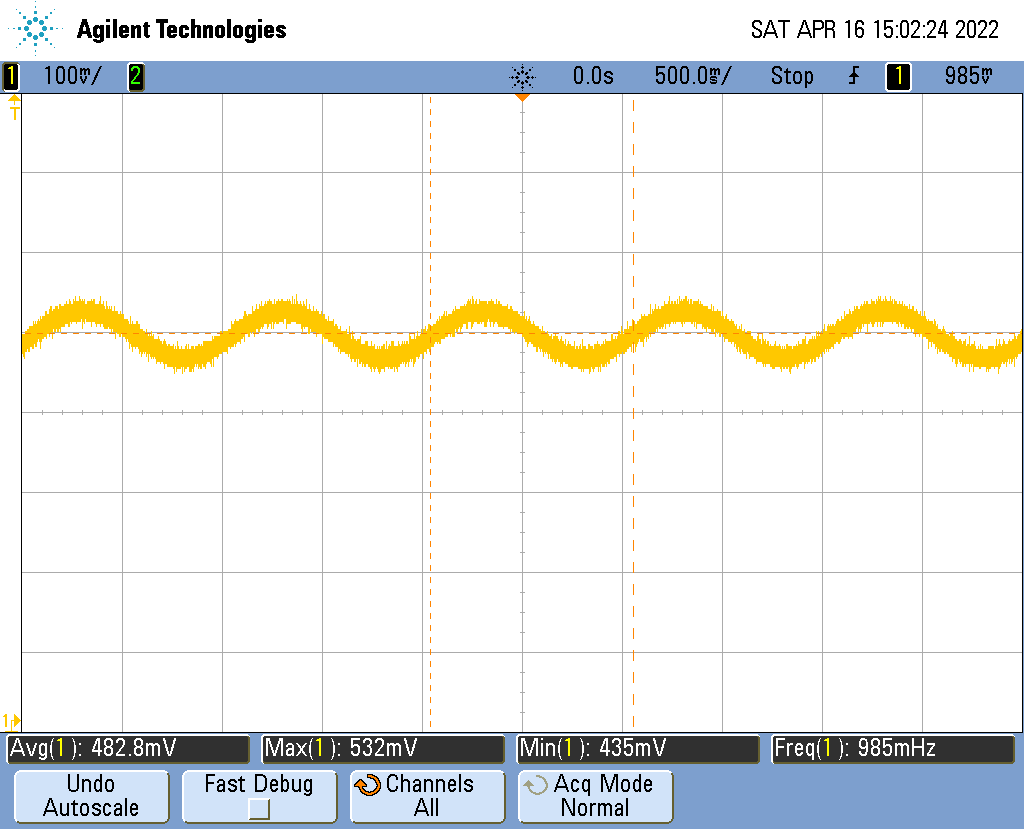
\includegraphics[width=8cm]{scope_0}
        \caption{Input signal \SI{482.8}{\milli\volt} DC offset and \SI{35}{\milli\volt}
        amplitude.}
        \label{fig:input}
	\end{figure}

	We can see the input signal from the signal generator in Figure \ref{fig:input}
	is about what we would expect out of the OPB745.
	The signal is quite noisy which manifests as "fuzz" on the
	oscilloscope capture. The next step is to apply a high pass filter to this signal
	to filter out the DC offset.

	\begin{figure}[h!]
        \centering
        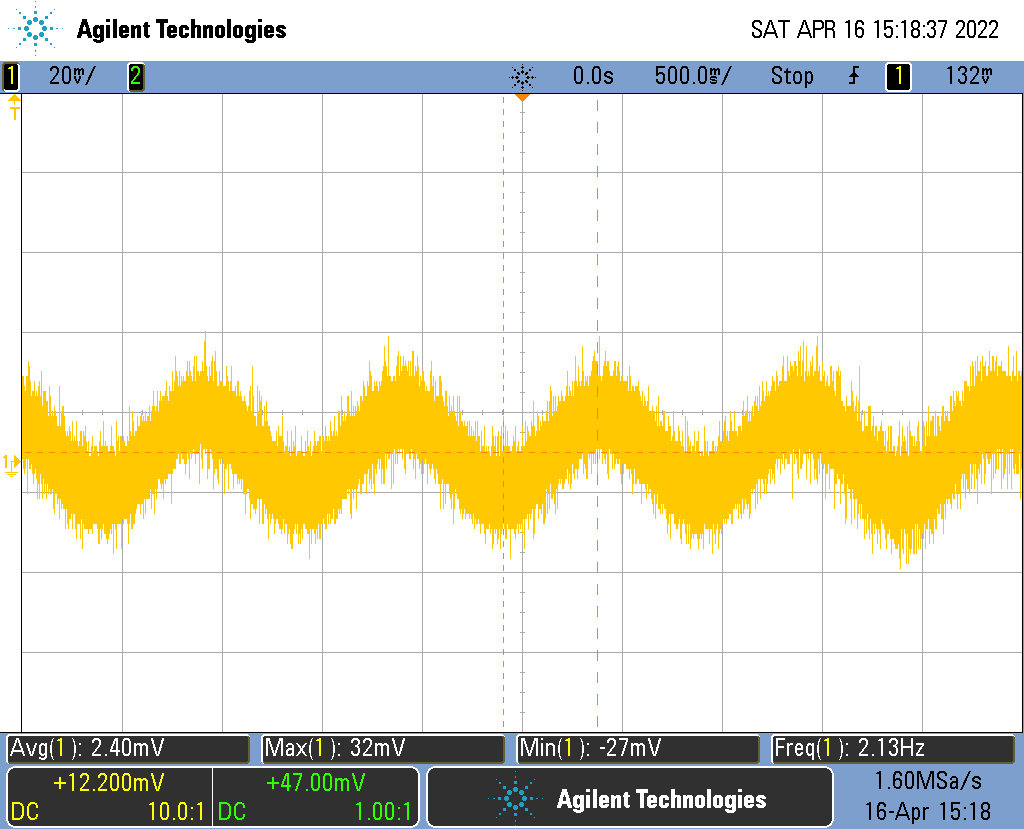
\includegraphics[width=8cm]{scope_2}
        \caption{Signal with high-pass filter applied.}
        \label{fig:high_pass}
	\end{figure}

	\pagebreak

	After applying a high pass filter, Figure \ref{fig:high_pass} shows the signal is
	now centered at
	\SI{0}{\volt} as expected. There is also a noticeable amplitude reduction to about
	\SI{20}{\milli\volt}. This feature will become important later on. Notice that the
	frequency detected by the oscilloscope is also incorrect at this stage because the
	presence of high amounts of noise will trip the trigger more. The next filter
	we must apply to this signal is a low pass to filter out the higher frequencies.

	\begin{figure}[h!]
        \centering
        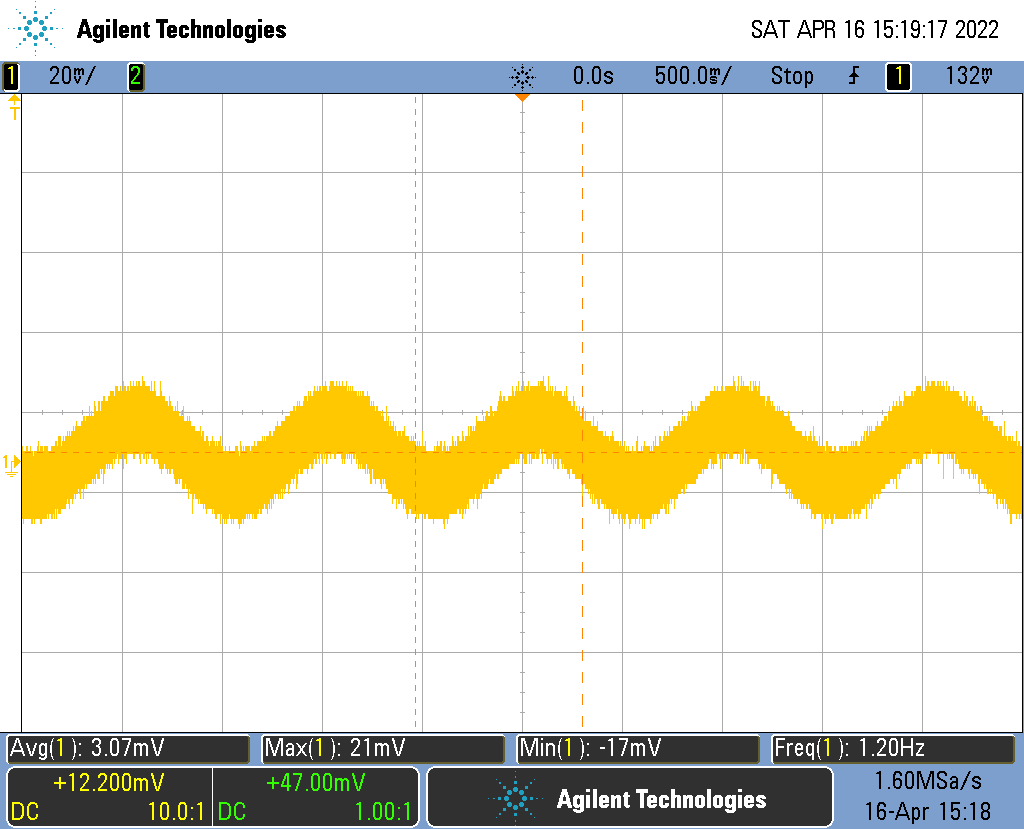
\includegraphics[width=8cm]{scope_3}
        \caption{Signal with high-pass and low-pass filters applied.}
        \label{fig:low_pass}
	\end{figure}

	Figure \ref{fig:low_pass} shows the signal with the high-pass and low-pass filters
	applied. We can see an improvement in the quality of the signal when comparing
	to Figure \ref{fig:high_pass}. The remaining fuzz is caused by the sampling error
	from the oscilloscope due to the a low signal amplitude. This will no longer be visible
	when the gain stage is applied.

	\pagebreak

	\begin{figure}[h!]
        \centering
        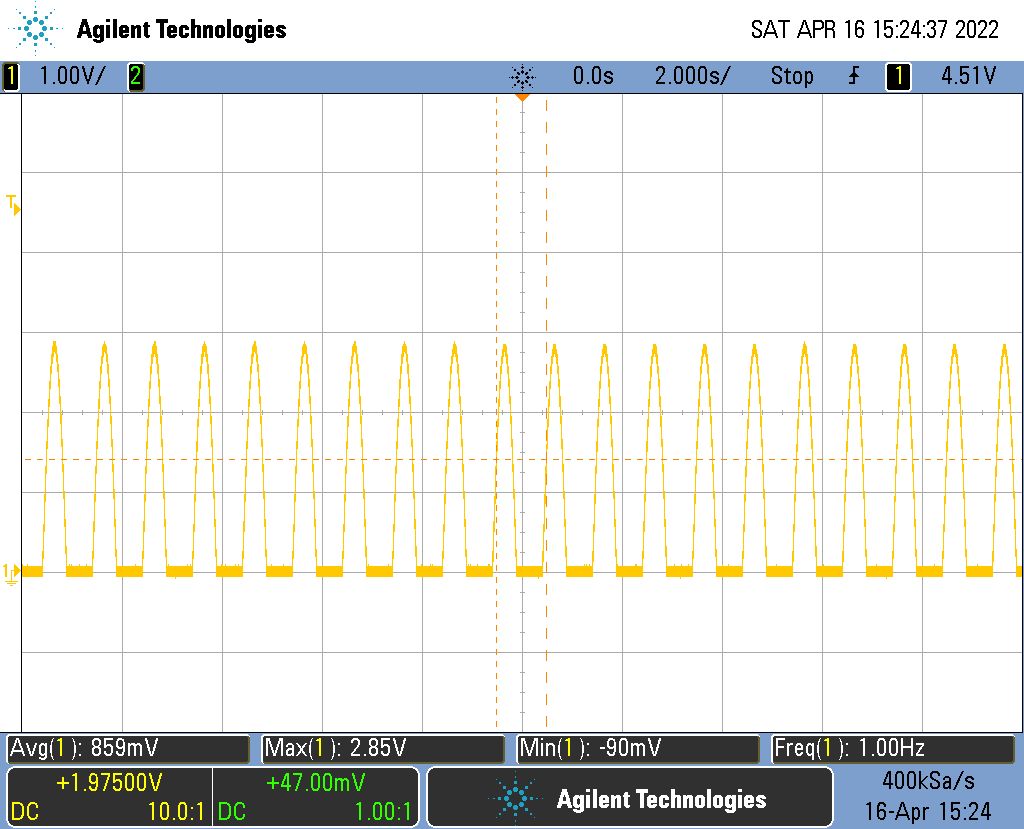
\includegraphics[width=8cm]{scope_4}
        \caption{Signal with high-pass, low-pass and gain stages applied.}
        \label{fig:gain}
	\end{figure}

	The generated signal shown in Figure \ref{fig:gain} is the ideal output to
	send to a micro-controller. There are some important features to note in the
	final signal. The simulation shows that the output of the circuit should have
	a gain of about \SI{44}{\dB}. At an output  amplitude of \SI{2.85}{\volt} and
	an input amplitude of \SI{35}{\milli\volt}, the actual gain about \SI{38.2}{\dB}.
	This may be due to dampening in low pass and high pass stages which is not modeled
	by the ideal components in the LT-spice simulation. Another feature of this wave
	when comparing it to the output of the low pass filter is the voltage cut off
	in the negative range. This occurs because the negative terminal on the op-amp
	is \SI{0}{\volt} and therefore cannot provide an output beyond this voltage.
	However, this characteristic of the signal will not effect the measurements
	discussed in the next section, as the micro-controller doesn't need both halves
	of the sine wave to estimate the frequency.\\

	There is one final step to protect the input pin
	on the ADC from being damaged. Too much current as well as voltage beyond the
	limits on the micro-controller will cause damage to the ADC peripheral. To avoid
	these two hazards, a \SI{100}{\ohm} resistor and two diodes are placed on the output
	node. The diodes are used to direct current to $V_{cc}$ or
	ground in case of a voltage surge or high amplitude input. The resistor is used to
	limit the current flow to the micro-controller and not overdrive the ADC peripheral.
	Figure \ref{fig:shotkey} shows the Shotkey protection circuit on the output
	of the gain stage.

	\begin{figure}[h!]
        \centering
        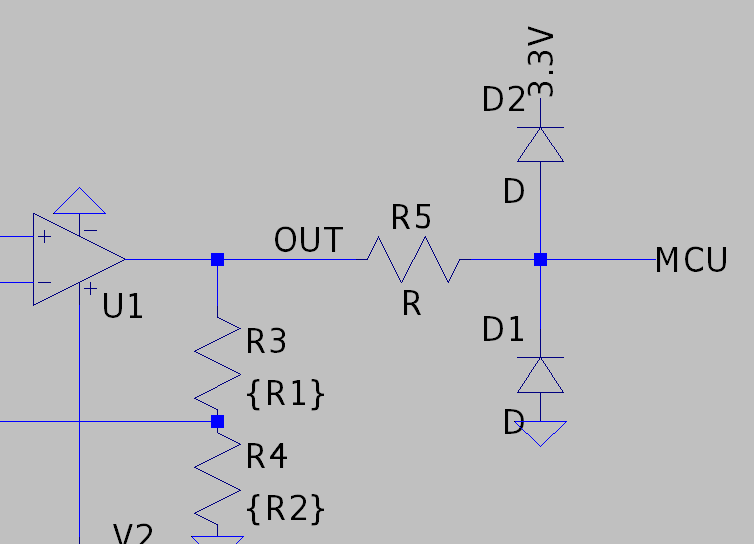
\includegraphics[width=8cm]{shotkey}
        \caption{Shotkey protection circuit for heartbeat sensor.}
        \label{fig:shotkey}
	\end{figure}

	The circuit shown in Figure \ref{fig:shotkey} is able to drive the circuit
	output to either \SI{0}{\volt} or \SI{3.3}{\volt} if the gain stage outputs
	beyond this range.

	\subsection*{Software}

	Once the circuit was constructed and verified to generate a clean signal, the
	next step was to use the micro-controller to measure the input frequency. To do
	this, the Analog-To-Digital converter (ADC) must be used to digitize the signal.
	The ADC driver written in \cite{b3} is used to perform this task. A simple way
	to find the frequency of a signal is to measure the time between rising edges.
	A rising edge can be classified as a transition from a low state to a high state.
	The simplest possible way to classify low states and high states is to provide a
	single threshold between low and high states. The issue with this approach in this
	application is that an extra rising edge may be detected if the signal were to
	jump slightly at the threshold due to noise. A single threshold is therefore extremely
	sensitive to noise and signal imperfections for this application.\\

	A more noise tolerant design is to use a Schmitt-trigger. The Schmitt trigger instead
	uses two thresholds. The upper threshold will send the system into a high state while
	the lower threshold will transition the system into a low state. The space in-between
	the two thresholds will hold the system state constant. This method is far more
	tolerant to small jumps and noise from the input signal and was used to find the
	rising edges while reading ADC values.\\

	To implement the actual data collection, a timer is used to trigger an ADC capture
	at a configurable frequency for a configurable length of time. Once enough data
	is collected, the timer is switched off and the system will average the distances
	between rising edges. Pressing one of the switches on the MSP432 will trigger
	the data collection cycle again.\\

	The software was tested using an upper threshold of \SI{1.5}{\volt} and a lower
	threshold of \SI{0.5}{\volt}. Input frequencies of \SI{3}{\hertz}, \SI{2}{\hertz},
	\SI{1}{\hertz}, and \SI{0.5}{\hertz} were tested to obtain an accurate set of readings
	over the full spectrum of heart rates we are interested in.

	\begin{figure}[h!]
        \centering
        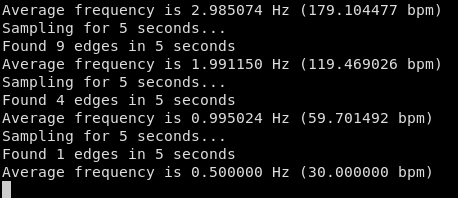
\includegraphics[width=8cm]{output}
        \caption{UART capture of software for \SI{3}{\hertz}, \SI{2}{\hertz},
	\SI{1}{\hertz}, and \SI{0.5}{\hertz} input signals.}
        \label{fig:output}
	\end{figure}

	Figure \ref{fig:output} shows the system responding to various input signals
	with the correct output. The output of the heartbeat monitor software proves
	the system has a fairly high degree of accuracy as it correctly displays the
	signal frequencies displayed on the signal generator.

	\subsection*{PCB}

	The final step of this lab exercise was to realize the schematic designed in
	PSpice as a printed circuit board (PCB) design in KiCAD. This process is fairly
	straight forward. The first step is to redraw the circuit schematic in KiCAD
	and assign part footprints to each component. The footprints will tell KiCAD the
	shapes and sizes of the terminals on the components in question. The next step
	is to layout the circuit components on the physical PCB. This can be tedious
	as avoiding crossing tracks can sometimes be problematic.

	\begin{figure}[h!]
        \centering
        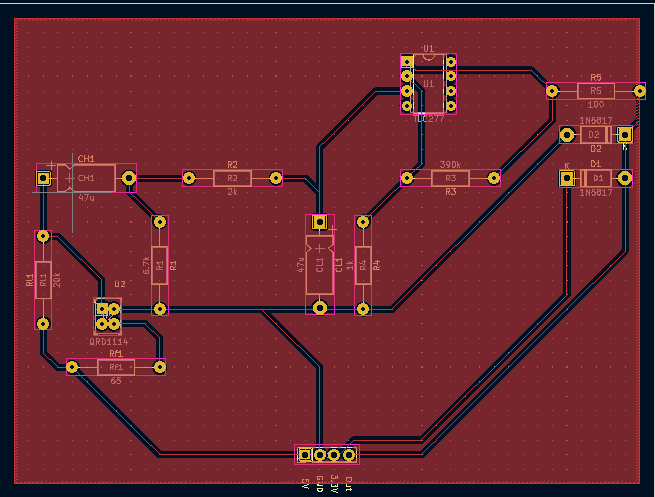
\includegraphics[width=8cm]{pcb}
        \caption{Physical layout of the heartbeat monitor circuit.}
        \label{fig:pcb}
	\end{figure}

	Figure \ref{fig:pcb} shows the physical layout of the PCB with all the
	relevant components in place. Although greater care could have been taken to
	constrain the overall size of the board, the main effort here was to attempt
	to match the layout of the schematic to the layout of the PCB. This would
	improve readability of the PCB itself even though not strictly required.
	We can see there are four pin headers exposed at the bottom of the PCB.
	These pins will interface with ground, \SI{5}{\volt}, \SI{3.3}{\volt} and
	the ADC input pin on the micro controller.

	\begin{figure}[h!]
        \centering
        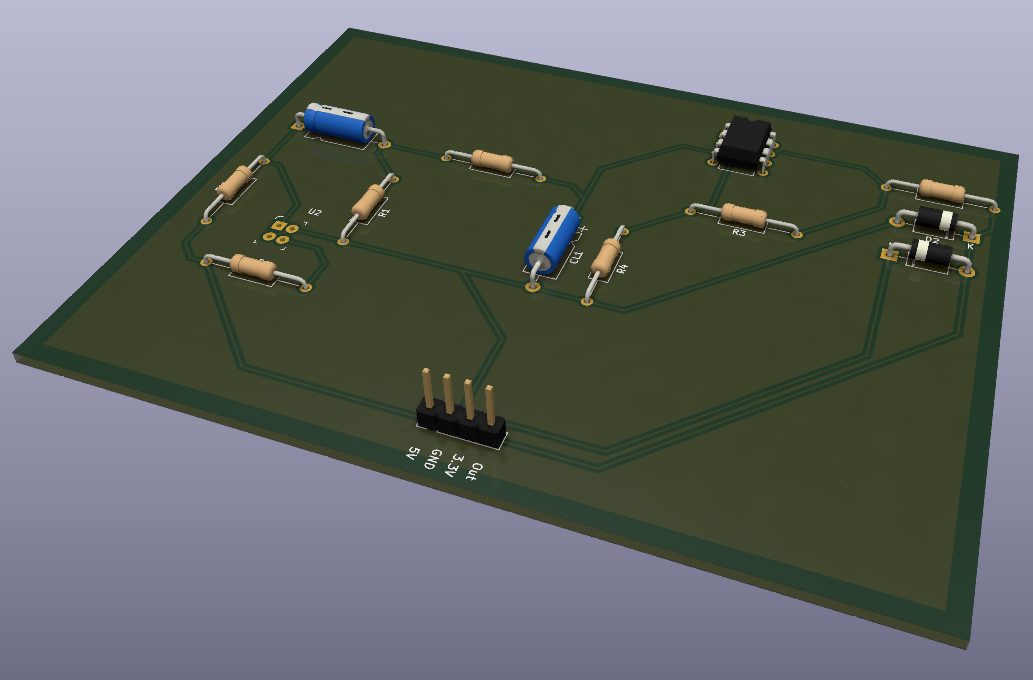
\includegraphics[width=8cm]{pcb_3d}
        \caption{3d rendering of the heartbeat monitor PCB.}
        \label{fig:pcb_3d}
	\end{figure}

	Figure \ref{fig:pcb_3d} shows a 3D view of the PCB with the components in place
	as well as labels for each of the four pin headers.

	\pagebreak

	The final step after designing and laying out the PCB is to place an order to
	the manufacturer. Most manufacturers accept a zip file containing a set of Gerber
	files and drill files describing the construction process of the PCB. KiCAD can
	generate these files once the design rules check has passed.

	\begin{figure}[h!]
        \centering
        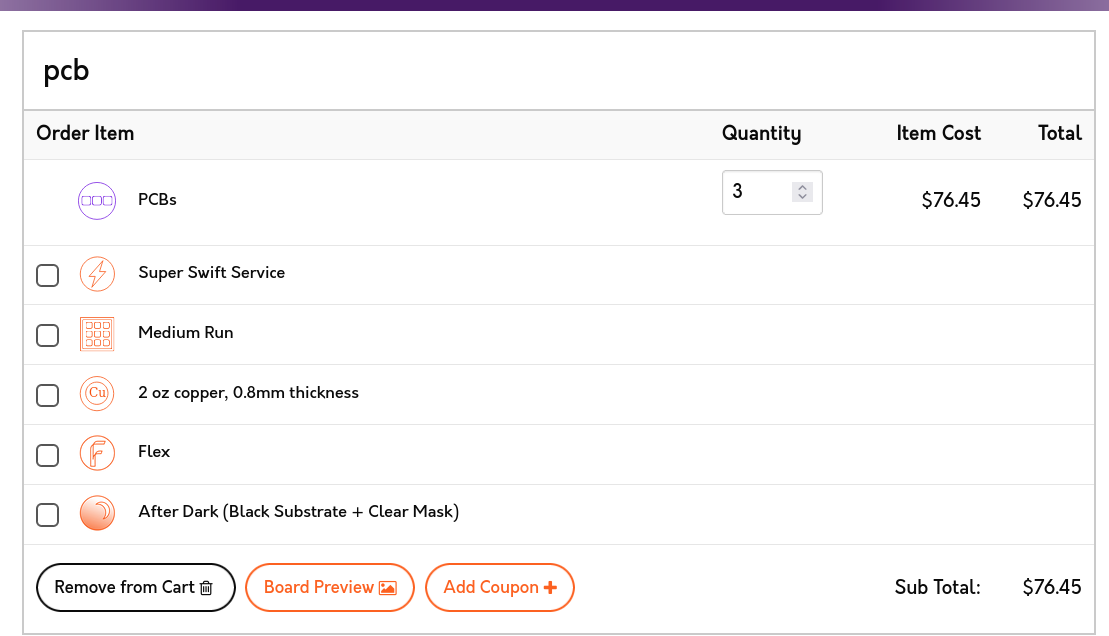
\includegraphics[width=8cm]{osh}
        \caption{3d rendering of the heartbeat monitor PCB.}
        \label{fig:osh}
	\end{figure}

	Figure \ref{fig:osh} shows an order ready to be placed for this PCB. This order
	is of course only for the PCB itself and not the components shown in the 3D view.
	These components must be ordered separately and soldered onto the PCB. A parts
	list was generated for the entire heartbeat monitor circuit.

\begin{table}[H]
    \renewcommand{\arraystretch}{1.2}
    \setlength{\tabcolsep}{12pt}
    \caption{Heartrate monitor parts list}
        \begin{center}
            \begin{tabular}{|c|c|c||c|c|}
                \hline
				Part & Quantity & Purpose\\\hline

\SI{65}{\ohm} Resistor			& 1	& Optoisolator input resistor\\\hline
\SI{20}{\kilo\ohm} Resistor		& 1	& Optoisolator output resistor\\\hline
OPB745							& 1	& Optoisolator sensor\\\hline
\SI{47}{\micro\farad} Capacitor	& 2	& High pass and low pass filters\\\hline
\SI{6.7}{\kilo\ohm} Resistor	& 1	& High pass filter\\\hline
\SI{2}{\kilo\ohm} Resistor		& 1	& Low pass filter\\\hline
\SI{390}{\kilo\ohm} Resistor	& 1	& Gain stage\\\hline
\SI{1}{\kilo\ohm} Resistor		& 1	& Gain stage\\\hline
TLC277							& 1	& Op-amp for gain stage\\\hline
\SI{100}{\ohm} Resistor			& 1	& Microcontroller current protection\\\hline
1N5817 Diode					& 2	& Microcontroller voltage protection\\\hline
            \end{tabular}
        \end{center}
        \label{tab:p1}
    \end{table}

	\section*{Questions}

	\begin{enumerate}
	\item
	The electrical rules check (ERC) and design rules check (DRC) are tools native
	to KiCAD that are meant to check certain characteristics of the schematic and
	PCB layout respectively. For example, the ERC will warn the designer of an
	unconnected terminal or component that is missing a footprint. The DRC will check
	physical design constraints such as a right angle track or a component being
	placed in close proximity to another component. These automated checks are not
	a ``catch-all'' for design mistakes but rather provide valuable insight to the
	designer on common issues.
	\item
	I originally designed the low pass filter with a cut-off frequency of \SI{7}{\hertz}.
	When I tested the signal on the breadboard, I found that the signal was still fairly
	noisy due to the low pass filter failing to filter out enough frequencies. I decided to
	drop the cutoff frequency to \SI{1.7}{\hertz}. Even though the upper limit of possible
	human heart rates are slightly above this frequency, the amplitude drop at the upper
	limit was low enough that the microcontroller did not experience any issues detecting
	rising edges in these signals.
	\item
	Interestingly, the gain did \emph{not} match the theoretical values. Specific values
	are discussed at length above. The main cause of this is that small variations in
	resistor and capacitor tolerance may have caused a negative gain in the filter stages.
	This negative gain would differ from the simulated circuit which would explain the
	discrepancy.
	\end{enumerate}

    \section*{Conclusion}

	This lab looked at filter design both in simulation as well as in reality on
	a physical breadboard. The passive components of the filter caused some issues in
	varying the gain slightly when comparing to the simulation. That was determined to
	be a tolerance related issue. This small variation in amplitude meant that the
	active gain stage needed to be adjusted to work properly with the physical
	components of the circuit. Once a clean signal with the proper characteristics
	was filtered and amplified, the microcontroller could detect a periodic signal
	using a noise tolerant Schmitt trigger design implemented in software. The Schmitt
	trigger worked very well as it correctly calculated the frequency of the input
	signal with a high degree of accuracy. Finally, the circuit was laid out on a PCB
	and a 

	\begin{thebibliography}{00}
\bibitem{b1} F. Arvin, S. Doraisamy, and E. Safar Khorasani, “Frequency shifting approach towards textual transcription of Heartbeat sounds,” Biological procedures online, 04-Oct-2011. [Online]. Available: https://www.ncbi.nlm.nih.gov/pmc/articles/PMC3396354/. [Accessed: 16-Apr-2022].
\bibitem{b2} B. Gholipour, “What is a normal heart rate?,” LiveScience, 13-Dec-2021. [Online]. Available: https://www.livescience.com/42081-normal-heart-rate.html. [Accessed: 16-Apr-2022].
\bibitem{b4} A. Tumbar, “Characterization of OPB745” Rochester Institute of Technology, 4-Feb-2022.
\bibitem{b3} A. Tumbar, “MSP432 Timers, Interrupts, and Analog-to-Digital Converter” Rochester Institute of Technology, 12-Feb-2022.
	\end{thebibliography}

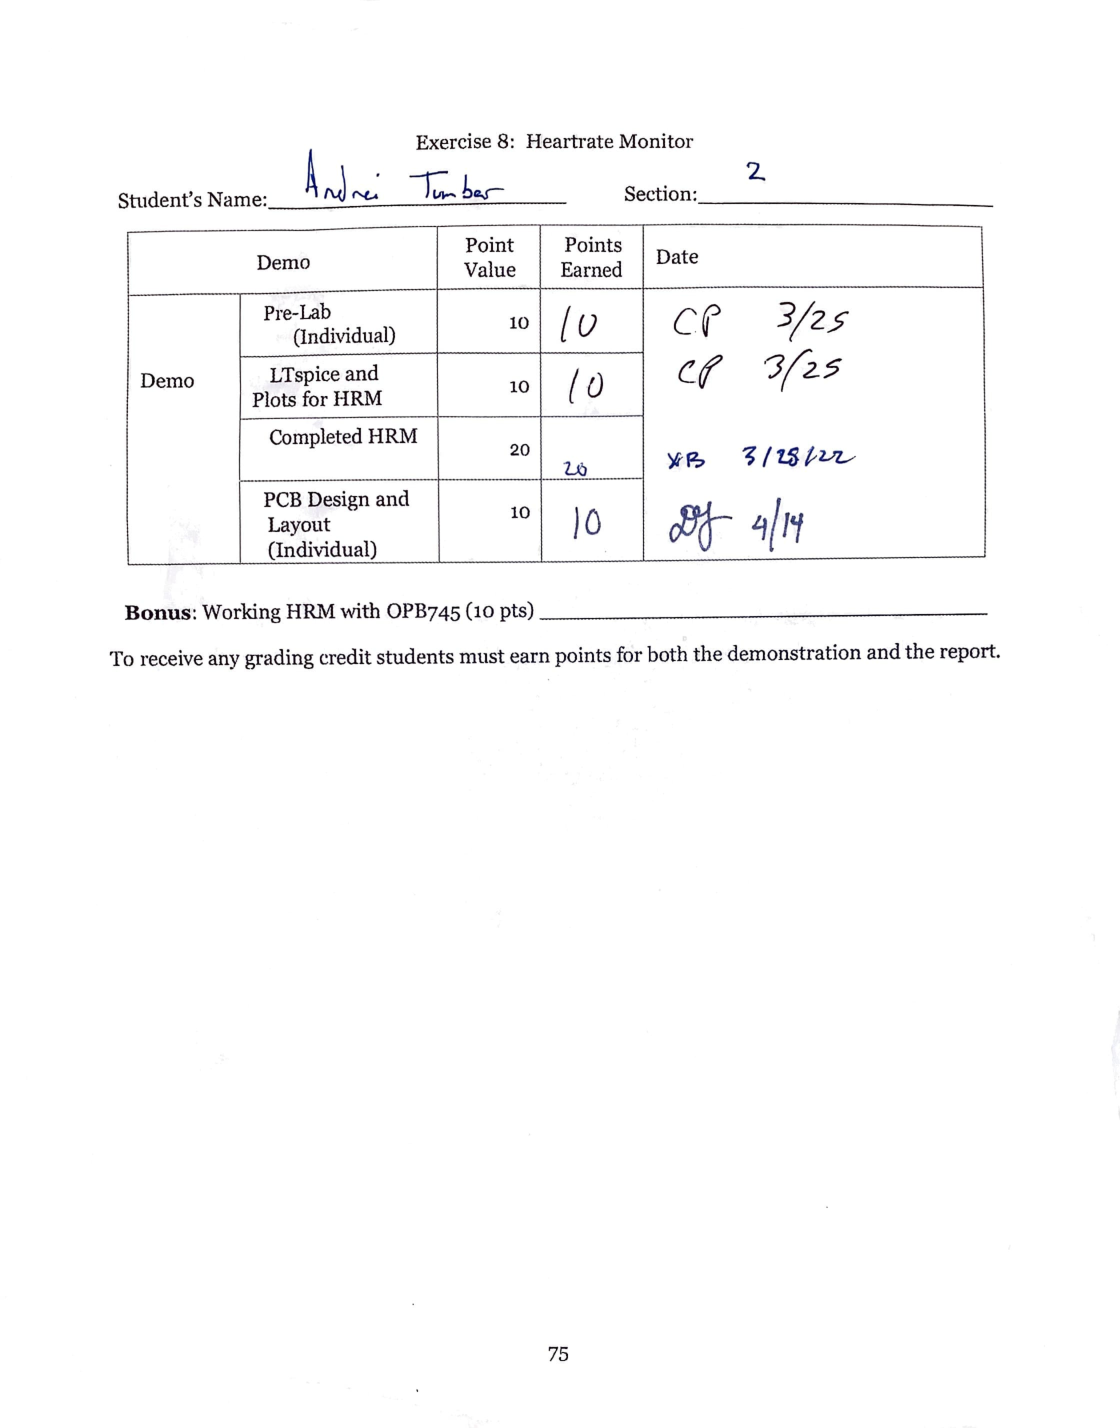
\includepdf[pages=-,pagecommand={},width=\textwidth]{signoff8.pdf}

\end{document}